\section{Dynamic Semantics with SDM}

The core idea when modelling behaviour is to regard dynamic aspects of a system
(let's call this a model as from now on) as bringing about a change of
state.
This means a model in state $S$ can evolve to state $S^*$ via a
transformation $\Delta: S \stackrel{\Delta}{\rightarrow}S^*$.
In this light, dynamic or behavioural aspects of a model are synonymous with
\emph{model transformations}, and the dynamic semantics of a language equate
simply to a suitable set of model transformations.
This approach is once again quite similar to OO where objects have state and can
\emph{do} things via methods that manipulate their state.        

So how do we model model transformations?  There are quite a few possibilities.
We could employ a suitably concise imperative programming language with which we
simply say in a step-by-step manner how the system morphs.
There actually exist quite a few very successful languages and tools in this
direction.

But isn't this almost like just programming directly in Java?
There must be a better way to do this\ldots  From the relatively mature
area of graph grammars and graph transformations we take a \emph{declarative}
and \emph{rule-based} approach.  
Declarative in this context means that we do not want to specify exactly how and
in what order changes to the model must be carried out to achieve a
transformation. 
We just want to say under what conditions the transformation can be executed
(precondition), and the state of the model after executing the transformation
(post condition). 
The actual task of going from precondition to postcondition should  be taken
over by a transformation engine and all related details are basically regarded
as a black box.         

Ok - so a model transformation is of the form $(pre, post)$.  Inspired by string 
grammars, let's call this black box transformation a \emph{rule}, and
consequently the precondition the left-hand side of the rule $L$ and the
postcondition the right-hand side $R$.  

A rule $r: (L,R)$ can be \emph{applied} to a model (a typed graph) $G$ by:
\begin{enumerate}
  \item Finding an occurrence of the precondition $L$ in $G$ via a \emph{match}
  $m$,
  \item Cutting out $Destroy := (L\setminus R)$ i.e., the elements that are
  present in the precondition but not in the postcondition are to be deleted,
  from $G$ to form  $(G\setminus Destroy)$ and
  \item Pasting $Create := (R\setminus L)$ i.e., new elements that are
  present in the postcondition but not in the precondition and are to be
  created, into the hole in $(G\setminus Destroy)$ to form a new graph $H =
  (G\setminus Destroy) \cup Create$.
\end{enumerate}

Rule application is denoted as $G \stackrel{r}{\Rightarrow} H$ and is depicted
in Fig.~\ref{fig:rule_application}. 

%\usepackage{graphics} is needed for \includegraphics
\begin{figure}[htp]
\begin{center}
  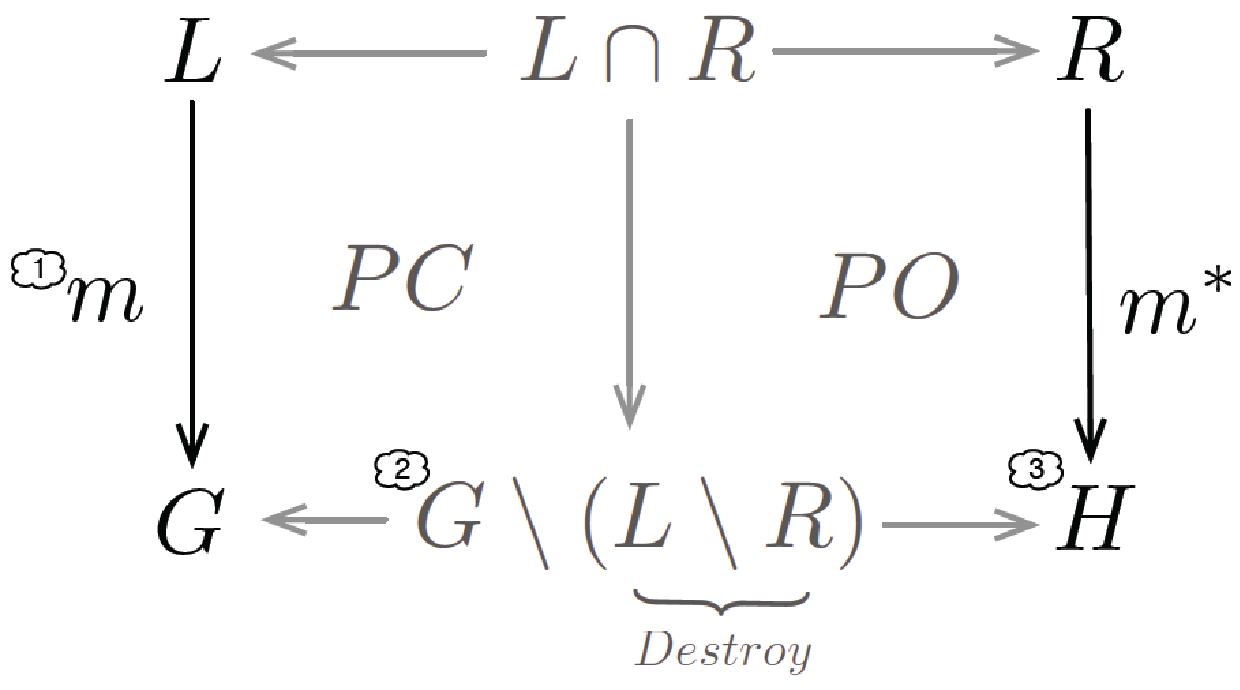
\includegraphics[width=0.6\textwidth]{pics/rule_application}
  \caption[]{Applying a rule $r: (L,R)$ to $G$ to yield $H$} 
  \label{fig:rule_application}
\end{center}
\end{figure}

(1) is called \emph{graph pattern matching}, (2) is called building a
\emph{push-out complement} $PC = (G\setminus Destroy)$, so that $L \cup
(G\setminus Destroy) = G$ and (3) is called building a \emph{push-out} $PO = H$,
so that $(G\setminus Destroy) \cup R = H$. A push-out is a generalised union
defined on typed graphs.  As we are dealing with graphs here, it is not such a
trivial task to define (1) -- (3) in precise terms with conditions when a rule
can be applied and not, and there exists substantial theory with exactly that
goal. As this formalisation of rule application involves two push-outs: one
(deletion) when cutting out $Destroy := (L\setminus R)$ from $G$ to yield
$(G\setminus Destroy)$, and one (creation) when inserting $Create := (R\setminus
L)$ in $(G\setminus Destroy)$ to yield $H$, this is referred to as a
\emph{double push-out}.  
We won't go into further details in this tutorial, but the interested reader can
refer to [Ref] for the exciting details.  

Now that we know what rules are, let's take a look at a simple example for our
memory box. How would a rule look like for moving a card from one partition to
the next?  Fig.~\ref{fig:rule_example} depicts the rule $moveCard$.

%\usepackage{graphics} is needed for \includegraphics
\begin{figure}[htp]
\begin{center}
  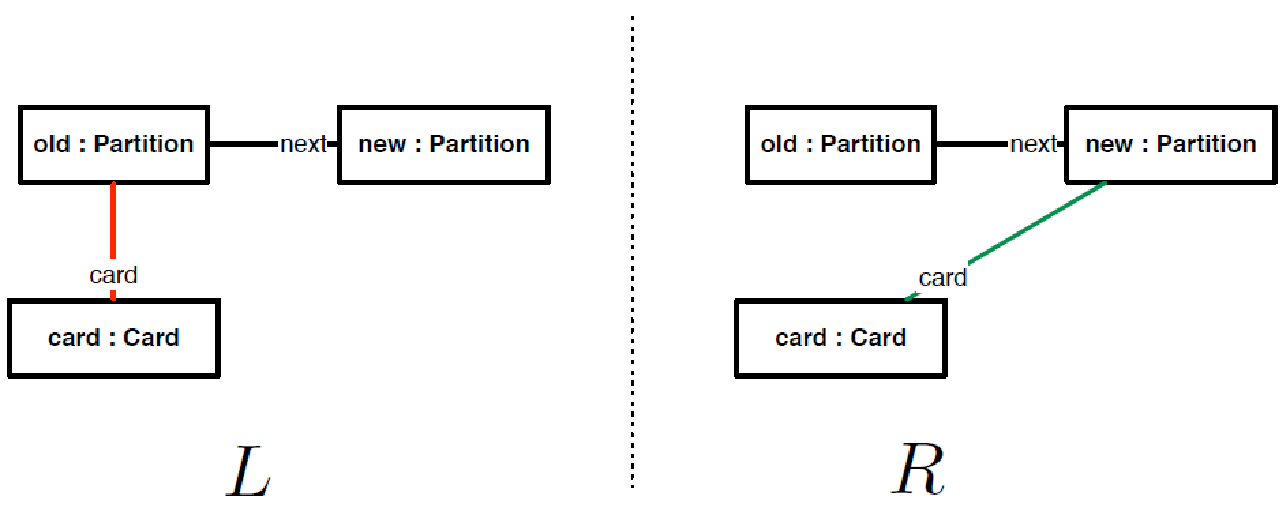
\includegraphics[width=0.9\textwidth]{pics/rule_example}
  \caption[]{Rule $moveCard$ as a graph transformation rule.}	
  \label{fig:rule_example}
\end{center}
\end{figure}

\clearpage

As already indicated by the colours used for $moveCard$ we employ a compact
representation of rules that is formed by merging $(L,R)$ into a single
\emph{story pattern} composed of  $Destroy := (L\setminus R)$ in red, $Retain := 
L\cap R$ in black, and $Create := (R\setminus L)$ in  green
(Fig.~\ref{fig:rule_compact}).
%\usepackage{graphics} is needed for \includegraphics
\begin{figure}[htp]
\begin{center}
  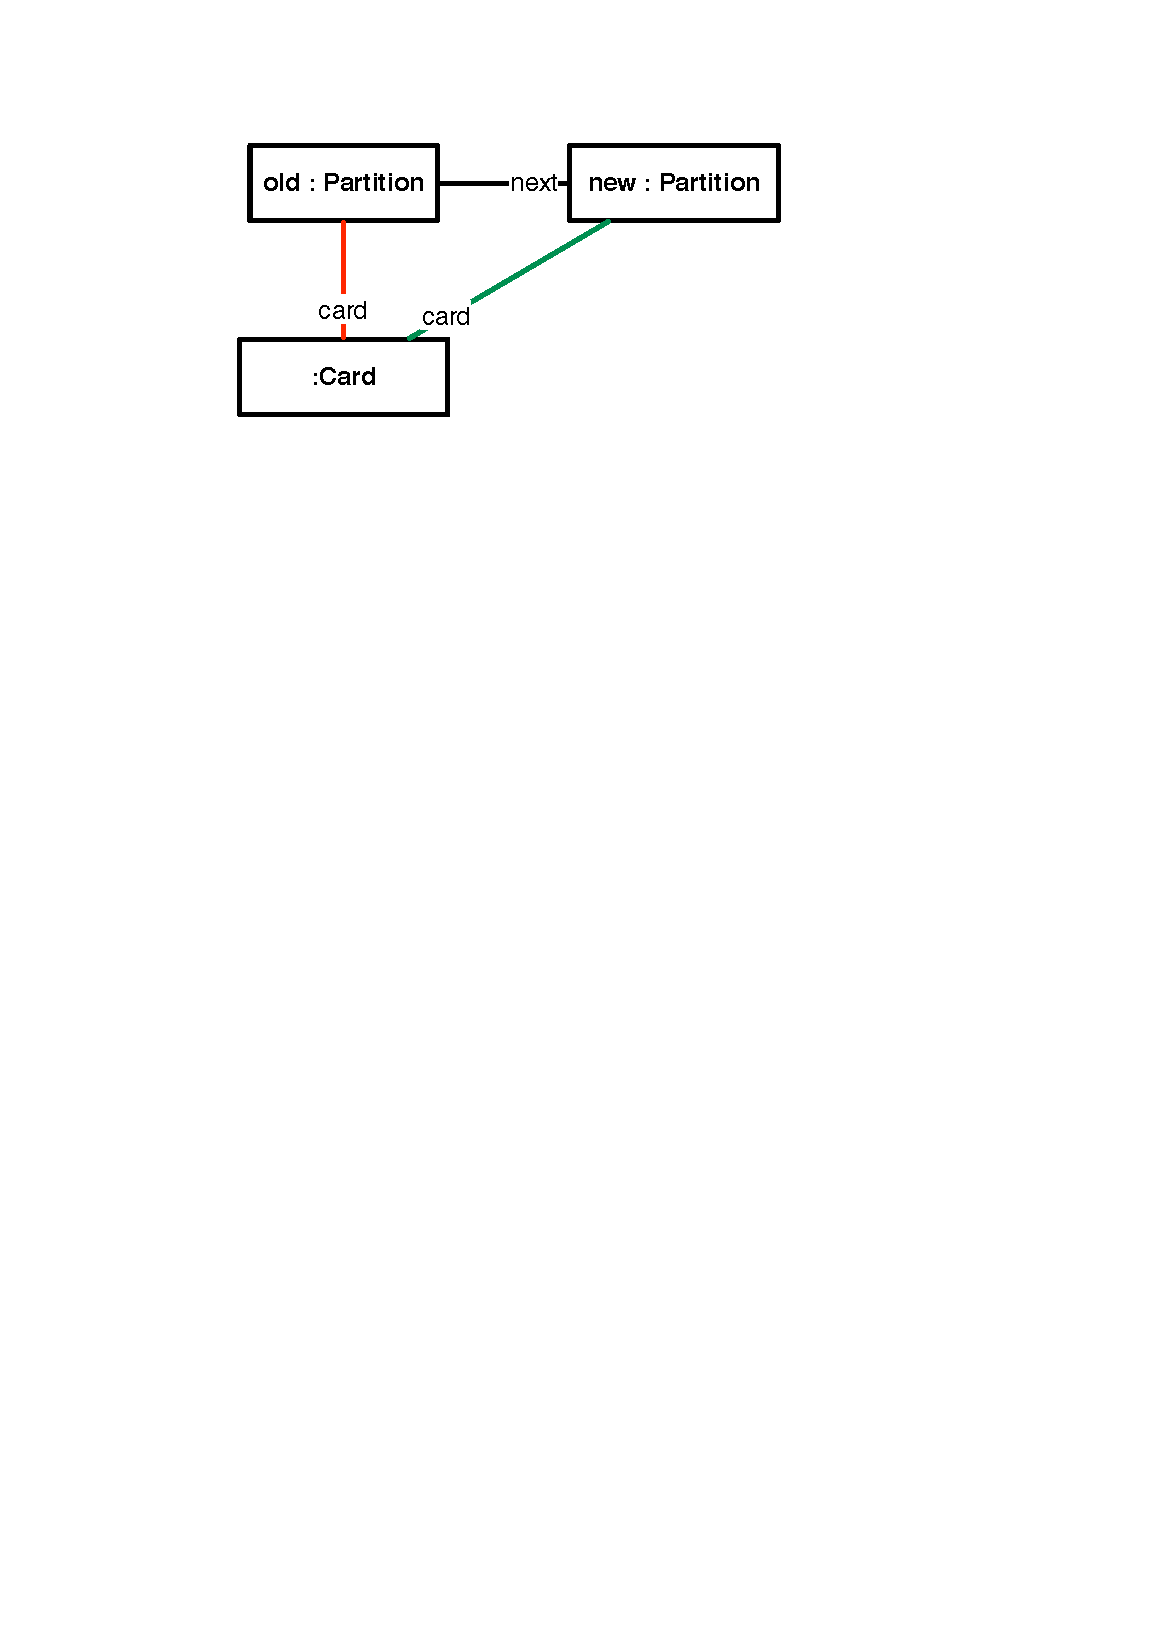
\includegraphics[width=0.45\textwidth]{pics/rule_compact}
  \caption[]{Compact representation of $moveCard$ as a Story Pattern.}
  \label{fig:rule_compact}
\end{center}
\end{figure}

 As we shall see in a moment, this  representation is quite intuitive and one can
just forget the details of rule application and think in terms of what is to be
deleted, retained and created. Applying $moveCard$ to a memory box according to
steps (1) -- (3) is depicted in Fig.~\ref{fig:rule_app_example}.

%\usepackage{graphics} is needed for \includegraphics
\begin{figure}[htp] 
\begin{center}
  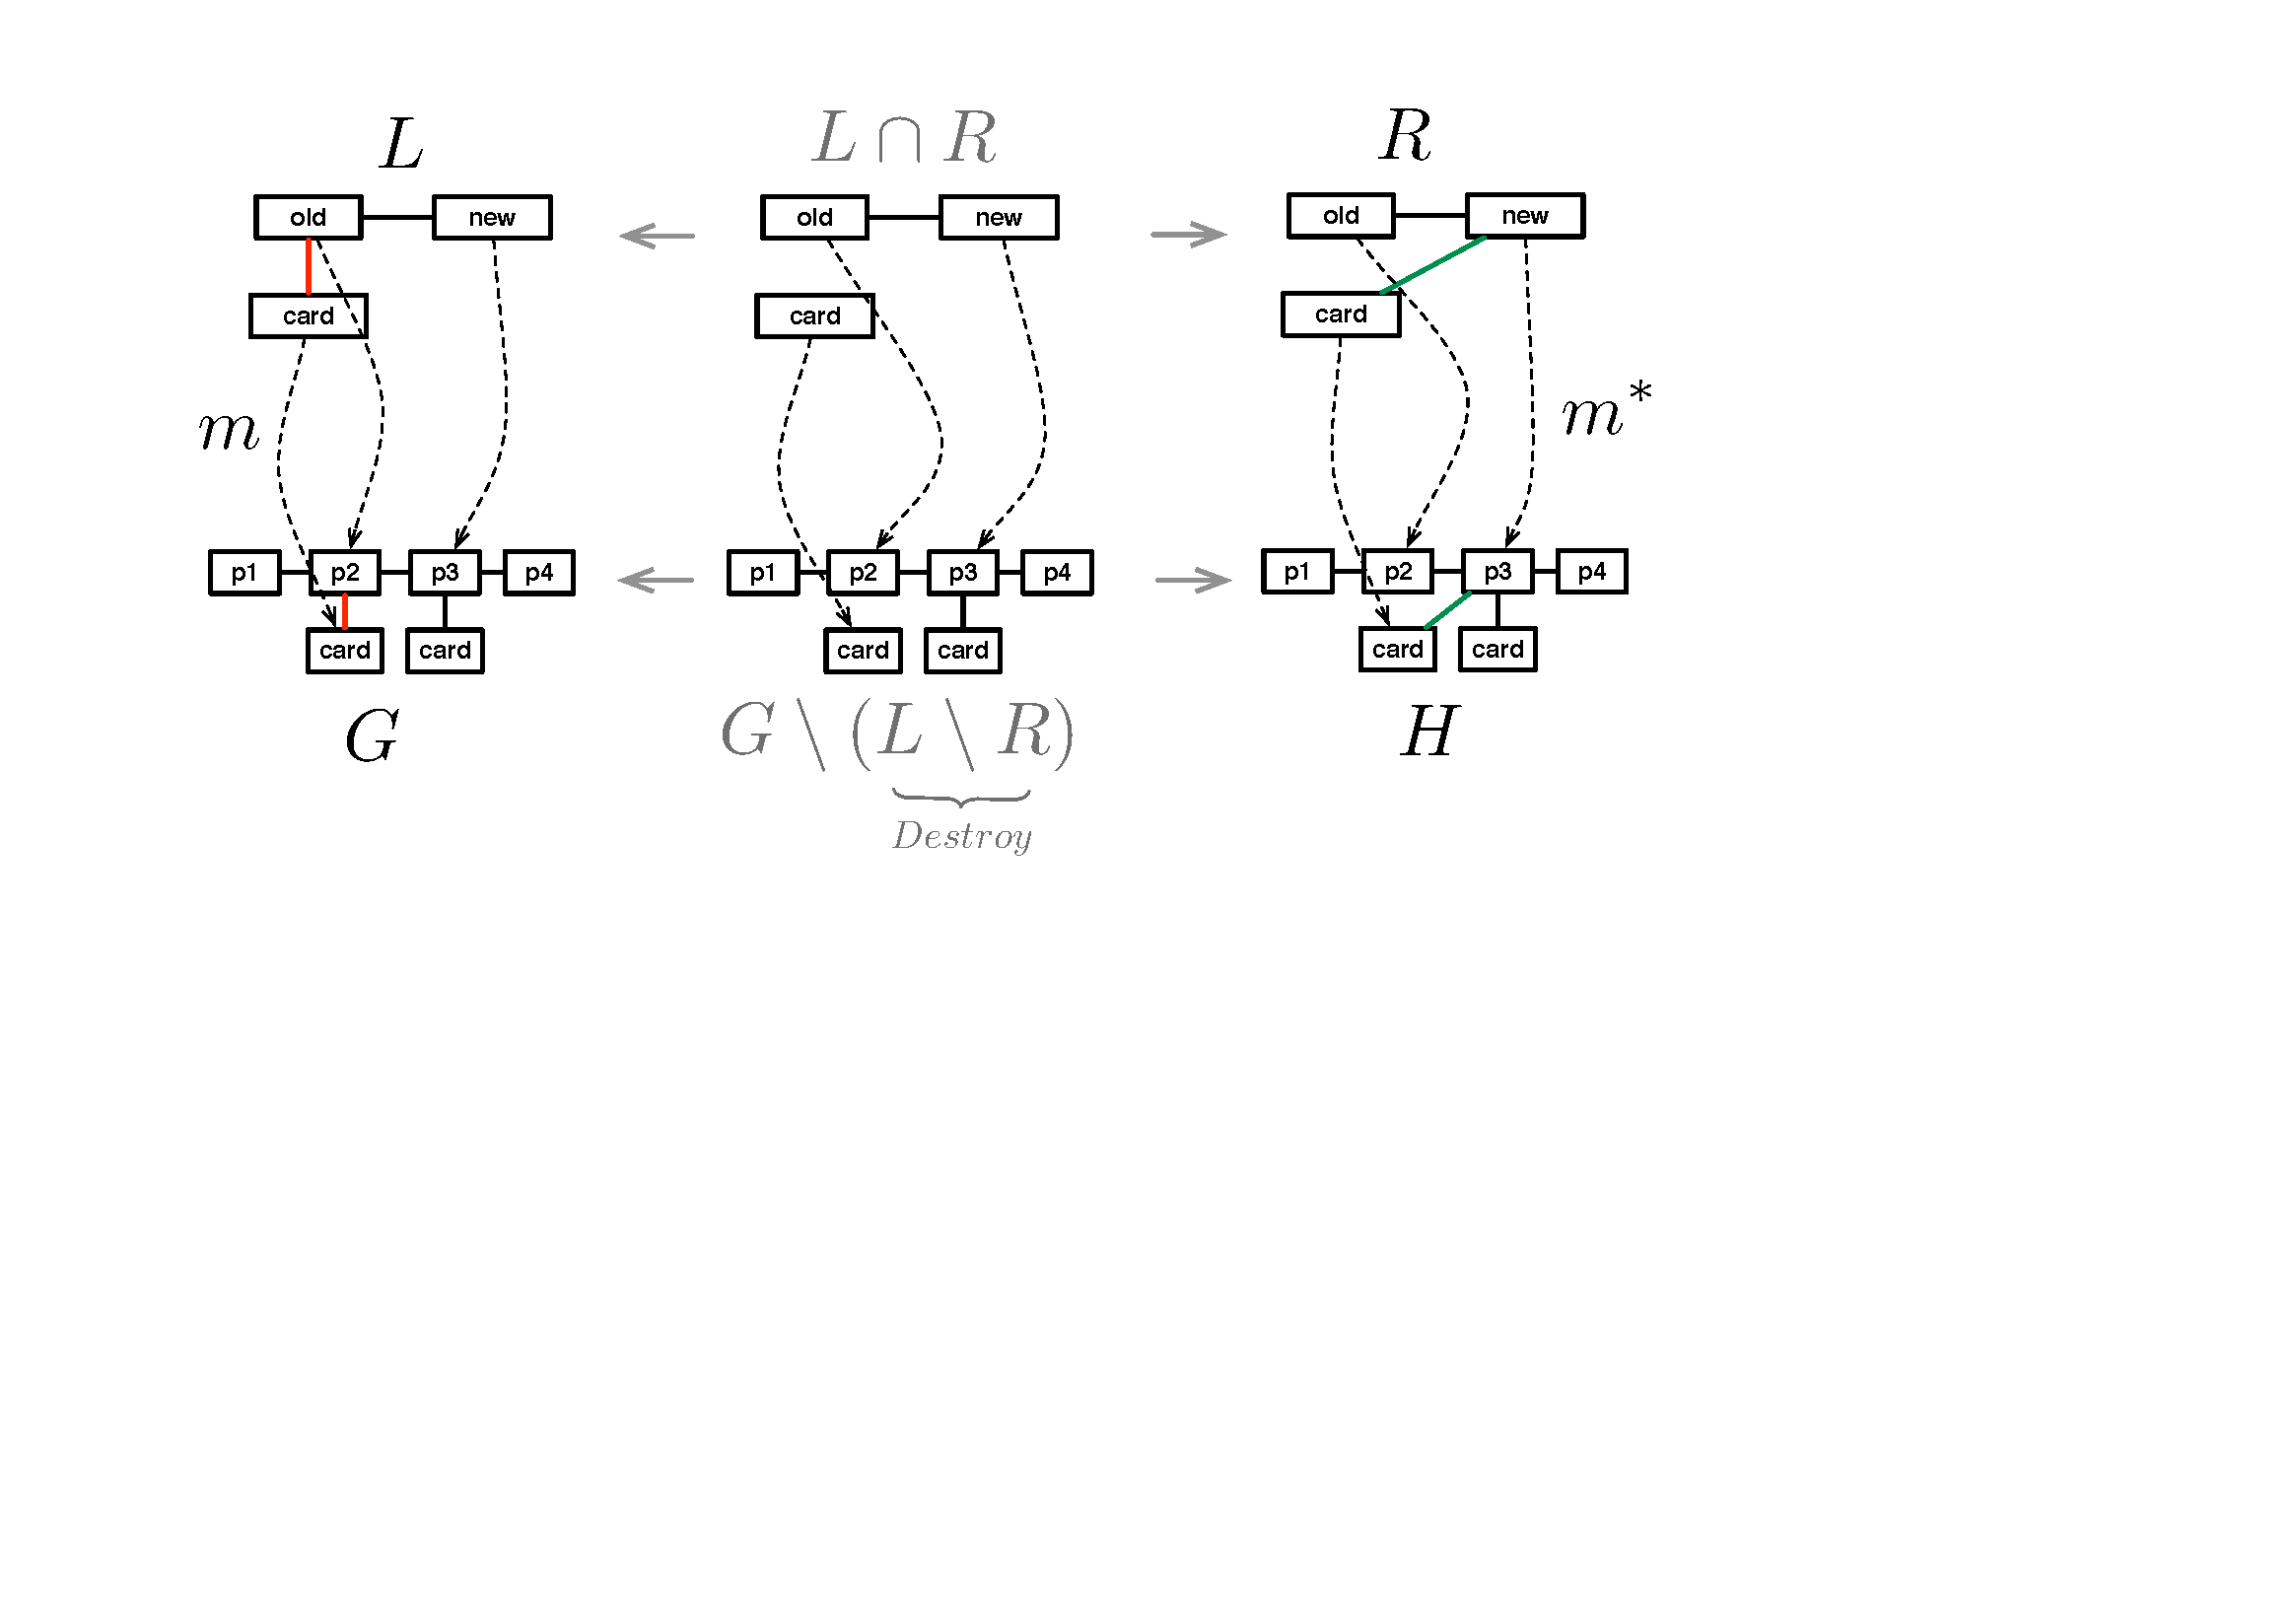
\includegraphics[width=\textwidth]{pics/rule_app_example}
  \caption[]{Applying $moveCard$ to a memory box.}
  \label{fig:rule_app_example}
\end{center}
\end{figure}

\clearpage 

One last thing before we continue with our memory box; individual rules still
have to be applied in a suitable sequence to realise complex model
transformations that consist of many steps.  This is realised with simplified
activity diagrams, where a single activity node is a pattern as discussed above,
and activity edges join nodes to form a control flow.   This can be viewed as
two layers:  an imperative layer to define the top-level control flow via
activity diagrams (if-else statements, loops etc), and a pattern layer
consisting of a story pattern in each activity node that specifies, via a graph
transformation rule, how the model is to be manipulated in that step.         

Enough theory! Grab your mouse and let's get cracking with SDMs\ldots